\newcommand{\cent}{{\mathrm{c}\mkern-9.0mu{/}}} %replaces \cent in math mode
\chapter{Mathematical Induction}


\newthought{As mentioned earlier}, to show that a proposition of
the form $\forall\,x\,P(x)$ is true, it is necessary to check that $P(c)$ is true
for every possible choice of $c$ in the domain of discourse. If that domain 
is not too big, it is feasible to check the truth of each $P(c)$ one by
one. For instance, consider the proposition {\it For every page in 
these notes,
the letter {\bfseries e} appears at least once on the page}. To express the 
proposition
in symbolic form we would let the domain of discourse be the set of pages in 
these
notes, and we would let the predicate $E$ be {\it has an occurrence of the
letter {\bfseries e}}, so the proposition becomes $\forall\,p\,E(p)$. The truth 
value of
this proposition can be determined by the tedious but feasible task of checking
every page of the notes for an {\bfseries e}. If a single page is found with no {\bf
e}'s, that page would constitute a counterexample to the proposition, and the
proposition would be false. Otherwise it is true.

When the domain of discourse is a finite set, it is, in principle, always
possible to check the truth of a proposition of the form $\forall\,x\,P(x)$ by
checking the members of the domain of discourse one by one. But that option is
no longer available if the domain of discourse is an infinite set since no
matter how quickly the checks are made there is no practical way to complete the
checks in a finite amount of time. For example, consider the proposition 
{\itshape For every natural number $n$, $n^5-n$ ends with a $0$}.%
\marginnote{Here the domain of 
discourse
is the set ${\N} = \{\,0,\,1,\,2,\,3,\,\cdots\}$.}%
The truth of the proposition could be established by checking: 
\begin{alignat*}{4}
 0^5-0 &= 0     &\quad 1^5-1 &= 0     &\quad 2^5-2   &=30     &\quad 3^5-3       &=240    \\
 4^5-4 &= 1020 &\quad 5^5-5  &= 3120  &\quad 6^5-6   &= 7770  &\quad 7^5-7    &=16800  \\
 8^5-8 &=32760 &\quad 9^5-9  &= 59040 &\quad 10^5-10 &= 99990 &\quad 11^5-11 &=161040 \\
 &\vdots&&\vdots&\vdots&&\vdots&
\end{alignat*}
\begin{center}
\itshape (and so on forever.)
\end{center}


Checking these facts one by one is obviously a hopeless task, and, of
course, just 
checking a few of them (or even a few billion of them) will never suffice to prove
they are all true. And it is not sufficient to check a few and say that the facts
are all clear. That's not a proof, it's only a suspicion. So verifying the truth
of  {\itshape $\forall\,n\,(n^5-n)$ ends with a $0$} for domain of discourse $\N$ seems tough.

\section{Mathematical induction}
In general, proving a universally quantified statement when the domain of
discourse is an infinite set is a tough nut to crack. But, in the special case
when the domain of discourse is the set $\N = \{\,0,\,1,\,2,\,3,\,\cdots\}$,
there is a technique called {\bfseries mathematical induction} that comes to the
rescue.
 
The method of proof by induction provides a way of checking
that all the statements in the list are true without actually verifying
them one at a time. The process is carried out in two steps. First (the
{\bfseries basis step}) we check that the first statement in the list is correct. 
Next (the 
{\bfseries inductive step}), we show that if any statement in the list is known 
to be
correct, then the one following must also be correct. Putting these two
facts together, it ought to appear reasonable that all the
statements in the list are correct. In a way, it's pretty amazing: we
learn infinitely many statements are true just by checking two facts. It's
like killing infinitely many birds with two stones.


So, suppose a list of statements, 
$p(0), p(1), p(2),\cdots, p(k), p(k+1)\cdots$ is presented and we want to show they are all true. 
The plan is to show two facts:
\begin{enumerate}
 \item $p(0)$ is true, and
 \item for any $n\in \N$, $p(n)\lra p(n+1)$.
\end{enumerate}
We then conclude all the statements in the list are true.

\section{The principle of mathematical induction}
The {\bfseries well ordering property} of the positive integers provides the
justification for proof by induction. This property asserts that every
non-empty subset of the natural numbers contains a smallest number. In fact, given
any nonempty set of natural numbers, we can determine the smallest number
in the set by the process of checking to see, in turn, if $0$ is in the set,
and, if the answer is {\itshape no}, checking for $1$, then for $2$, and so on.
Since the set is nonempty, eventually the answer will be {\itshape yes, that
number is in the set}, and in that way, the smallest natural number in the
set will have been found. Now let's look at the proof that induction is a valid
form of proof. The statement of the theorem is a little more general than 
described above. Instead of beginning with a statement $p(0)$, we allow
the list to begin with a statement $p(k)$ for some integer $k$ (almost always,
$k=0$ or $k=1$ in practice). This does not have any effect of the concept
of induction. In all cases, we have a list of statements, and we show the
first statement is true, and then we show that if any statement is true, so is the
next one. The particular name for the starting point of the list doesn't really matter.
It only matters that there is a starting point.


\begin{thm}[Principle of Mathematical Induction]  
Suppose we have a list of statements %\hfill\break 
$p(k), p(k+1), p(k+2),\cdots, p(n), p(n+1)\cdots$. 
\begin{enumerate}
 \item $p(k)$ is true, and
 \item $p(n)\lra p(n+1)$ for every $n\geq k$,
\end{enumerate}
then all the statements in the list are true.
\end{thm}
\begin{proof}
 The proof will be by contradiction.
 
 Suppose that 1 and 2 are true, but that it is not the case that $p(n)$ 
 is true for all $n\geq k$.
 Let $S=\{n | n\geq k \text{ and } p(n) \text{ is false}\}$, so that 
  $S\neq \emptyset$.
 Since $S$ is a non-empty set of integers $\geq k$
  it has a least element, say
 $t$. So $t$ is the
 smallest positive integer for which $p(n)$ is false.
 In the ever colorful jargon of mathematics, $t$ is usually
 called the {\itshape minimal criminal}.
 
 Since $p(k)$ is true, $k\notin S$. Therefore $t>k$. 
 So $t-1\geq k$.
 Since $t$ is the smallest integer $\geq k$ for which $p$ is false,
 it must be that   $p(t-1)$ is true. 
 Now, by part 2, we also know $p(t-1)\to p(t)$ is true. So it must be that
 $p(t)$ is true, and that is a contradiction.
\end{proof}

\section{Proofs by induction}
Many people find proofs by induction
a little bit black{-}magical at first, but just keep the goals in mind
(namely check [1] the first statement in the list is true,
and [2] that if any statement in the list is true, so is the one that
follows it) and the process won't seem so confusing.

A handy way of viewing mathematical induction is to compare proving the sequence 
$p(k)\land p(k+1)\land p(k+2)\land ...\land p(m)\land ...$ to knocking down
a set of dominos set on edge and numbered consecutively $k,k+1,....$. If we want to knock all of the 
dominos down, which are numbered $k$ and greater, then we must knock the
$k$th domino down, and ensure that the spacing of the dominos is such that every
domino will knock down its successor. If either the spacing is off ($\exists m\geq k$
with $p(m)$ not implying $p(m+1)$), or if we fail to knock down the $k$th domino (we do not
demonstrate that $p(k)$ is true), then there may be dominos left standing.
\marginnote{%
When checking the inductive step, $p(n)\to p(n+1)$, the
statement $p(n)$, is called the {\bfseries inductive hypothesis}.
}%

To discover how to prove the inductive step most people start by explicitly listing
several of the first instances of the inductive hypothesis $p(n)$. Then, look for how
to make, in a general way, an argument from one, or more, instances to the next instance
of the hypothesis.  Once an argument is discovered that allows us to advance from the truth
of previous one, or more, instances, that argument, in general form, becomes the pattern for
the proof on  the inductive hypothesis. Let's examine an example.

\clearpage
\begin{exmp}
 Let's prove that, for each positive integer $n$, 
the sum of the first $n$ positive integers is $\displaystyle \frac{n(n+1)}{2}$.
Here is the list of statements we want to verify:
\begin{align*}
 p(1):\quad   & 1 = \frac{1(1+1)}{2}  &\text{add $2$ to both sides, can you make $p(2)$ appear?}\\
 p(2):\quad   & 1+2 = \frac{2(2+1)}{2} &\text{add $3$ to both sides,  can you make $p(3)$ appear?}\\
 p(3):\quad   & 1+2+3 = \frac{3(3+1)}{2} \\
              &\vdots \\
 p(n):\quad   & 1+2+\cdots+n = \frac{n(n+1)}{2} \\
 p(n+1):\quad & 1+2+\cdots+(n+1) = \frac{(n+1)((n+1)+1)}{2} \\
              &\vdots
\end{align*}
Once you figure out the general form of the argument%
\sidenote{For this example it will be some calculation}%
 that takes us from one instance of $p(\cdot)$ to the next, you have form of the inductive argument.

\begin{proof}
 \textsf{Basis:} Let's check the first statement in the list,\\
 $\displaystyle p(1): \quad 1 = \frac{1(1+1)}{2}$,
  is correct. The left-hand side is $1$, and the right-hand side is
 $\displaystyle \frac{1(1+1)}{2}= \frac{2}{2} = 1$, so the two sides are equal
 as claimed.
 
 \textsf{Inductive Step:} Suppose $p(n)$ is true for some integer $n\geq 1$.
 In other words, suppose
  $1+2+\cdots+n = \frac{n(n+1)}{2}$. We need to show $p(n+1)$ is true.
 In other words, we need to verify 
 $1+2+\cdots+(n+1) = \frac{(n+1)((n+2)}{2}$.
 Here are the computations:%
 \marginnote{To prove an equality, the usual strategy is to start on one side of the
 equation, $p(n+1)$ in this case, obtain the other side. We do this
  through a series of algebraic manipulations and
 using the general induction hypothesis, $p(n)$, along the way.}
 \begin{align*}
  1+2+\cdots+(n+1) &= 1+2+\cdots+n+(n+1) \\
  & = \frac{n(n+1)}{2} + (n+1) \text{ using the inductive hypothesis} \\
  & = \frac{n(n+1)}{2} + \frac{2(n+1)}{2} \\
  & = \frac{n(n+1) + 2(n+1)}{2} \\
  & = \frac{(n+1)(n+2)}{2}
 \end{align*}
 as we needed to show. So we conclude all the statements in the list are true.
\end{proof}
\end{exmp}

\section{Examples}
The next example reproves the useful formula for the sum of the terms in a geometric
sequence. Recall that to form a geometric sequence, fix a real number $r\not=1$, and list
the integer powers of $r$ starting with $r^0=1$: $1,r,r^2,r^3,\cdots, r^n,\cdots$.
The formula given in the next example shows the result of adding
$1+r+r^2+\cdots r^n$.

\begin{exmp} For all $n\geq 0$, we have
$\displaystyle{\sum_{k=0}^n r^k = \frac{r^{n+1}-1}{r-1}}$, (if $r\not=1$).\marginnote{In this %
example, $p(n)$ is the statement: 
\[\displaystyle p(n): \sum_{k=0}^n r^k = \frac{r^{n+1}-1}{r-1}\].}

\begin{proof}[by induction on $n$:] (We assume $r\not=1$.)

\textsf{Basis:}
When $n=0$ we have 
$\displaystyle{\sum_{k=0}^0 r^k = r^0 = 1}$. We also have 

$\displaystyle \frac{r^{n+1}-1}{r-1} = \frac{r-1}{r-1}=1$.


\textsf{Inductive Step:} 
Now suppose that  $\displaystyle \sum_{k=0}^n r^k = \frac{r^{n+1}-1}{r-1}$ is true for some $n\geq 0$.
Then, we see that
\begin{align*}
 \sum_{k=0}^{n+1} r^k &= \left(\sum_{k=0}^n r^k\right) + r^{n+1}\quad
                              \text{ by the recursive definition of a sum} \\
                      &= \frac{r^{n+1}-1}{r-1} + r^{n+1}\quad \text{ by inductionhypothesis}, \\
                      &= \frac{r^{n+1}-1}{r-1}+\frac{r^{n+2}-r^{n+1}}{r-1}  \\
                      &= \left[\frac{r^{n+1}-1+r^{n+2}-r^{n+1}}{r-1}\right]  \\
                      &= \frac{r^{n+2}-1}{r-1}.
\end{align*}
\end{proof}
\end{exmp}

\begin{exmp} For every integer $n\geq 2$, $2^n>n+1$.
\begin{proof}
 \textsf{Basis:} When $n=2$, the inequality to check is $2^2>2+1$, and that
 is correct.
 
 \textsf{Inductive Step:} Now suppose that $2^n>n+1$ for some integer $n\geq 2$.
 Then $2^{n+1} = 2\cdot 2^n> 2(n+1) = 2n + 2 >n+2$, as we needed to show.
\end{proof}
\end{exmp}

\clearpage
\begin{exmp} Show that using only $5\cent$ stamps and  $9\cent$
stamps,
any postage amount $32\cent$ or greater can be formed.
\begin{proof}
 \textsf{Basis:}  $32\cent$ can be formed by using one $5\cent$ stamp
 and three $9\cent$ stamps.
 
 \textsf{Inductive Step:} Now suppose we can form $n\cent$ postage for some
 $n\geq 32$. We need to show we can form $(n+1)\cent$ postage.
 Since $n\geq 32$, when we form  $n\cent$ postage, we must use either
 (1) at least seven $5\cent$ stamps, or (2) at least one  $9\cent$ 
 stamps. For if both of those possibilities are wrong, we will have at most
 $30\cent$ postage.
 
 \textsf{case 1:} If there are seven (or more) $5\cent$ stamps in the 
 $n\cent$ postage, remove seven $5\cent$, and put in 
 four $9\cent$ stamps. Since we removed $35\cent$ and
 put back $36\cent$, we now have  $(n+1)\cent$ postage.
 
 \textsf{case 2:} If there is one (or more)  $9\cent$ stamps in the
 $n\cent$ postage, remove one  $9\cent$, and put back
 two $5\cent$. Since we removed  $9\cent$ and put back
  $10\cent$, we now have $(n+1)\cent$ postage.
 
 So, in any case, if we can make  $n\cent$ postage for some
 $n\geq 32$, we can form $(n+1)\cent$ postage. Thus, by induction,
 we can make any postage amount  $32\cent$ or greater.
\end{proof}
\end{exmp}

\begin{exmp}
 Let's now look at an example of an induction proof with a geometric flavor. Suppose we
 have a $4\times 5 $ chess board:
 
 \begin{marginfigure}
   \resizebox{\textwidth}{!}{
  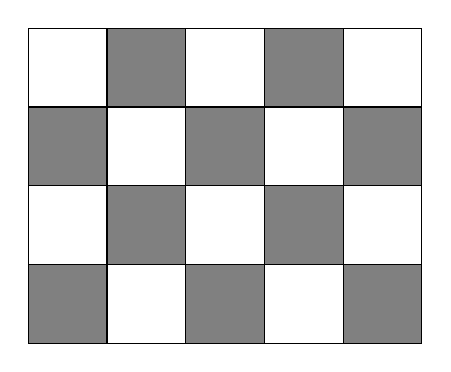
\begin{tikzpicture}
  
      \pgfmathsetmacro{\hboardsize}{5}
      \pgfmathsetmacro{\vboardsize}{4}
  
      \foreach \i in {1,...,\hboardsize}{
          \foreach \j in {1,...,\vboardsize}{
              \pgfmathsetmacro{\weight}{(1 + (-1)^(\i+\j))*50};
              \node[draw,rectangle,fill=gray!\weight,minimum size=1cm] (node\i-\j) at (\i,\j) {};
          }
      }
    \end{tikzpicture}
   } %end resizebox
   \caption{$4\times 5$ chessboard}
 \end{marginfigure}

 
 and a supply of $1\times 2$ dominos:
% \includegraphics[scale=0.10]{Graphics/Domino.png}
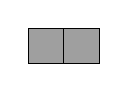
\begin{tikzpicture}[scale=0.45,transform shape]
    \node[draw,rectangle,fill=gray!75,minimum size=1cm] (nodeA) at (1,1) {};
    \node[draw,rectangle,fill=gray!75,minimum size=1cm] (nodeB) at (2,1) {};
  \end{tikzpicture}

 
 Each domino covers exactly two squares on the board. A {\bfseries perfect cover} of
 the board consists of a placement of dominos on the board so that each domino
 covers two squares on the board (dominos can be either vertically or horizontally
 orientated), no dominos overlap, no dominos extend beyond the edge of the board,
 and all the squares on the board are covered by a domino. It's easy to see that
 the $4\times 5$ board above has a perfect cover. More generally, it is not
 hard to prove:
 
 \begin{thm}
  An $m\times n$ board has a perfect cover with $1\times 2$ dominos  if and only
  if at least one of $m$ and $n$ is even.
 \end{thm} 
\end{exmp}


\begin{exmp} Now consider a $2^n\times 2^n$ board for $n$ a positive integer.
Suppose somewhere on the board there is one {\itshape free square} which does not have to
be covered by a domino. For $n=3$ the picture could appear as in figure \ref{fig:8x8 board},
where the shaded square is the free square.
 \begin{marginfigure}
 \resizebox{\textwidth}{!}{
  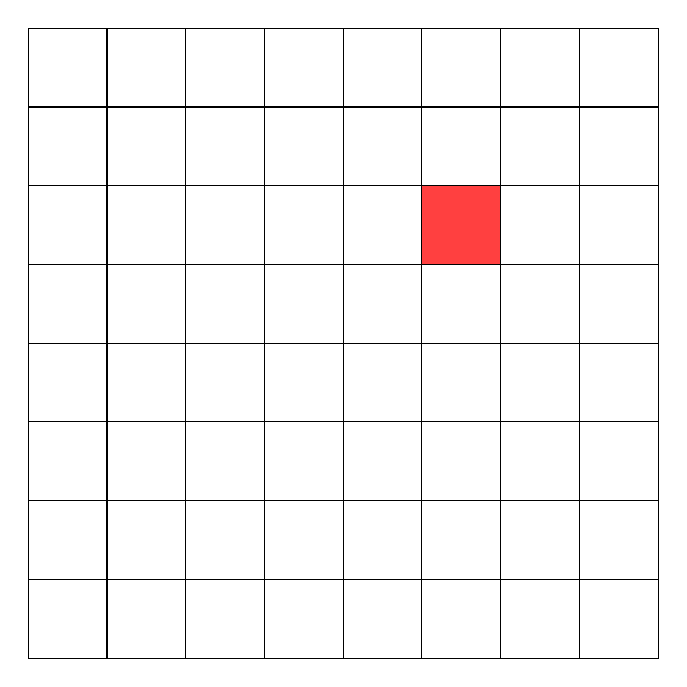
\begin{tikzpicture} 
      \pgfmathsetmacro{\hboardsize}{8}
      \pgfmathsetmacro{\vboardsize}{8}
  
      \foreach \i in {1,...,\hboardsize}{
          \foreach \j in {1,...,\vboardsize}{
              \pgfmathsetmacro{\weight}{(1 + (-1)^(\i+\j))*50};
              \node[draw,rectangle,minimum size=1cm] (node\i-\j) at (\i,\j) {};
          }
      }
      \node[draw,rectangle,fill=red!75,minimum size=1cm] (nodeX) at  (6,6) {};
      
    \end{tikzpicture}
  } %end resizebox
  \caption{$2^3\times 2^3$ chessboard}\label{fig:8x8 board}
 \end{marginfigure}


This time we have a supply of $L$-shaped dominos:
%\includegraphics[scale=0.10]{Graphics/Ldomino.png}
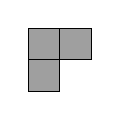
\begin{tikzpicture}[x=0.40cm,y=0.40cm]
    \node[draw,rectangle,fill=gray!75,minimum size=0.40cm] (node1) at (1,1) {};
    \node[draw,rectangle,fill=gray!75,minimum size=0.40cm] (node2) at (1,2) {};    
    \node[draw,rectangle,fill=gray!75,minimum size=0.40cm] (node3) at (2,2) {};
\end{tikzpicture}
These dominos (which can be rotated) each cover exactly three squares on the board.
We will prove by induction that every such board has a perfect cover using
$L$-shaped dominos.
\begin{proof}
 \textsf{Basis:} For $n=1$, the board to cover is an $L$-shaped domino, so
 it certainly has a perfect cover.
 
 \textsf{Inductive Step:} Assume now that for some integer $n\geq 1$, 
 any $2^n\times 2^n$ with one free square can be perfectly covered by
 $L$-shaped dominos. Consider a $2^{n+1}\times 2^{n+1}$ board with one free square.
 Divide the board in half horizontally and vertically. Each quarter of the
 board will be a  $2^n\times 2^n$ board, and one of those quarters
 will have a free square in it (see figure \ref{fig:8x8 board}).
 \begin{marginfigure}
  \resizebox{\textwidth}{!}{
   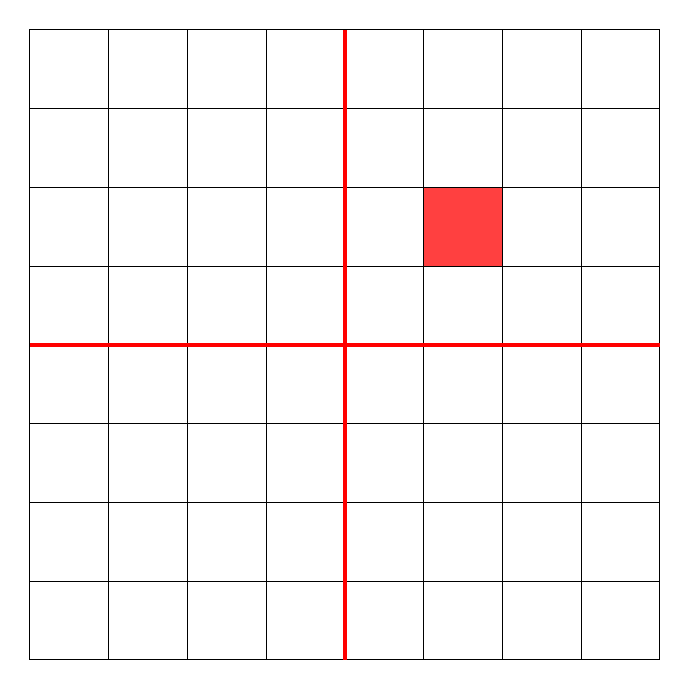
\begin{tikzpicture} 
       \pgfmathsetmacro{\hboardsize}{8}
       \pgfmathsetmacro{\vboardsize}{8}
   
       \foreach \i in {1,...,\hboardsize}{
           \foreach \j in {1,...,\vboardsize}{
               \pgfmathsetmacro{\weight}{(1 + (-1)^(\i+\j))*50};
               \node[draw,rectangle,minimum size=1cm] (node\i-\j) at (\i,\j) {};
           }
       }
       %draw excluded square
       \node[draw,rectangle,fill=red!75,minimum size=1cm] (nodeX) at  (6,6) {};
       %draw dividing lines
       \draw[red, ultra thick] (4.5,0.5) -- (4.5,8.5);
       \draw[red, ultra thick] (0.5,4.5) -- (8.5,4.5);
             
     \end{tikzpicture}
   } %end resizebox
   \caption{Divided $2^3\times 2^3$ chessboard}\label{fig:8x8 board divided}
  \end{marginfigure}
 
 We now add one $L$-shaped domino as shown in figure \ref{fig:8x8 board with domino}.
  \begin{marginfigure}
   \resizebox{\textwidth}{!}{
    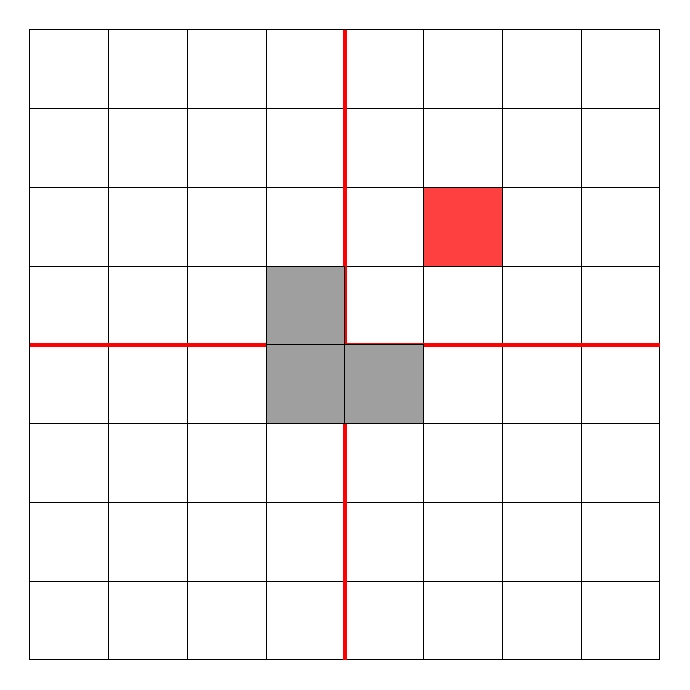
\begin{tikzpicture} 
        \pgfmathsetmacro{\hboardsize}{8}
        \pgfmathsetmacro{\vboardsize}{8}
    
        \foreach \i in {1,...,\hboardsize}{
            \foreach \j in {1,...,\vboardsize}{
                \pgfmathsetmacro{\weight}{(1 + (-1)^(\i+\j))*50};
                \node[draw,rectangle,minimum size=1cm] (node\i-\j) at (\i,\j) {};
            }
        }
        %draw excluded square
        \node[draw,rectangle,fill=red!75,minimum size=1cm] (nodeX) at  (6,6) {};
        %draw dividing lines
        \draw[red, ultra thick] (4.5,0.5) -- (4.5,8.5);
        \draw[red, ultra thick] (0.5,4.5) -- (8.5,4.5);
        %place domino
        \node[draw,rectangle,fill=gray!75,minimum size=1cm] (node1) at (4,5) {};
        \node[draw,rectangle,fill=gray!75,minimum size=1cm] (node1) at (4,4) {};    
        \node[draw,rectangle,fill=gray!75,minimum size=1cm] (node1) at (5,4) {};
              
      \end{tikzpicture}
    } %end resizebox
    \caption{$2^3\times 2^3$ board with domino}\label{fig:8x8 board with domino}
   \end{marginfigure}

 
 This leaves us with essentially four  $2^n\times 2^n$ boards, each
 with one free square. So, by the inductive assumption, they can each
 be perfectly covered by the $L$-shaped dominos, and so the entire
 board can be perfectly covered.
\end{proof}
\end{exmp}

\section{Second principle of mathematical induction}
There is a second version of mathematical induction. Anything that can be proved
with this second version can be proved with the method described above, and vice versa,
but this second version is often easier to use. The change occurs in the induction
assumption made in the inductive step of the proof.
The inductive step of the method described above ($p(n)\to p(n+1)$ for all $n\geq k$)
is replaced with
$[p(k)\land p(k+1)\land \cdots\land p(n)]\to p(n+1)$ for all $n>k$. The effect is that
we now have a lot more hypotheses to help us derive $p(n+1)$.
In more detail, the second form of mathematical induction is described in the following theorem.
\ms
\begin{thm}[Second Principle of Mathematical Induction]
\  \\
 For integers $k$ and $n$, if
 \begin{enumerate}
   \item $p(k)$ is true, and
   \item $[p(k)\land p(k+1)\land ...\land p(n)]\to p(n+1)$ for an arbitrary $n\geq k$,
 \end{enumerate}
 then $p(n)$ is true for all $n\geq k$.
\end{thm}

This principle is shown to be valid in the same way the first form of induction was justified.
The utility lies in dealing with cases where we want to use inductive reasoning,
but cannot deduce the $(n+1)$st case form the $n$th case directly. Let's do  a few
 examples
of proofs using this second form of induction. One more comment before doing the examples.
In many induction proofs, it is convenient to check several initial cases in the basis step to
avoid having to include special cases in the inductive step. The examples below illustrate
this idea.
\ms

\begin{exmp}
 Show that using only $5\cent$ stamps and  $9\cent$
 stamps,
 any postage amount $32\cent$ or greater can be formed.
 \begin{proof}
 \ \\
  \textsf{Basis:} We can certainly make
   \begin{align*}
     32\cent &= (1)5 \cent+ (3)9\cent \\
     33\cent &= (3)5 \cent+ (2)9\cent \\
     34\cent &= (5)5 \cent+ (1)9\cent \\
     35\cent &= (7)5 \cent+ (0)9\cent \\
     36\cent &= (0)5 \cent+ (4)9\cent 
   \end{align*}  
   \textsf{Inductive Step:} Suppose we can make all postage amounts from $32\cent$
   up to some amount $k\cent$ where $k\geq 36$. Now consider the problem
   of making $(k+1)\cent$. We can make $(k+1-5)\cent= (k-4)\cent$ 
   postage since $k-4$ is between $32$ and $k$. Adding a  $5\cent$ stamp to
   that gives the needed  $k+1\cent$ postage.
 \end{proof}
 
\end{exmp}

In that example, the basis step was a little messier than our first solution to the problem, but
to make up for that, the inductive step required much less cleverness.
 
 
\begin{exmp}
 Induction can be used to verify a guessed closed from formula
 for a recursively defined sequence. Consider the sequence defined recursively by
 the initial conditions $a_0=2$, $a_1=5$ and the recursive rule, for $n\geq 2$, 
 $a_n = 5a_{n-1} - 6a_{n-2}$. The first few terms of this sequence
 are $2,5, 13, 35, 97,\cdots$. A little experimentation leads to the guess
 $a_n = 2^n+3^n$. Let's verify that guess using induction. For the basis of the
 induction we check our guess gives the correct value of $a_n$ for $n=0$ and $n=1$.
 That's easy. For the inductive step, let's suppose our guess is correct up to $n$ where
 $n\geq 2$. Then, we have
 \begin{align*}
   a_{n+1} &= 5a_n-6a_{n-1} \\
           &= 5(2^{n}+3^{n}) -6(2^{n-1}+3^{n-1}) \\
           & = (5\cdot2-6)2^{n-1} - (6-5\cdot3)3^{n-1} \\
           & = 4\cdot2^{n-1} - (-9)\cdot3^{n-1} \\
           & = 2^{n+1}+3^{n+1} \text{  as we needed to show.}
 \end{align*}
\end{exmp} 


\begin{exmp}
 In the game of {\bfseries Nim}, two players are presented with a
 pile of matches. The players take turns removing one, two, or three matches at a time.
 The player forced to take the last match is the loser. For example, if the pile initially
 contains $8$ matches, then first player can, with correct play, be sure to win.
 Here's how: player 1: take $3$ matches leaving $5$; player 2's options will leave
 $4, 3,$ or $2$ matches, and so player 1 can reduce the pile to $1$ match on her turn,
 thus winning the game. Notice that if player 1 takes only $1$ or $2$ matches on her
 first turn, she is bound to lose to good play since  player 2 can then reduce the pile to
 $5$ matches.
 
 Let's prove that if the number of matches in the pile is $1$ more than a multiple of $4$, the
 second player can force a win; otherwise, the first player can force a win.
 \begin{proof}
  For the basis, we note that obviously the second player wins if there is $1$ match in the pile,
 and for $2,3$, or $4$ matches the first player wins by taking $1,2$, or $3$ matches in each case,
 leaving $1$ match.
 
 For the inductive step, suppose the statement we are to prove is correct for the number of
 matches anywhere from $1$ up to $k$ for some $k\geq4$. Now consider a pile of $k+1$
 matches. 
 
 \textsf{case 1:}
 If $k+1$ is $1$ more than a multiple of $4$, then when player 1 takes her matches,
 the pile will {\ub {not}} contain $1$ more than a multiple of $4$ matches, and so the next player
 can force a win by the inductive assumption. So player 2 can force a win.
 
 \textsf{case 2:} If $k+1$ is not $1$ more than a multiple of $4$, then player 1 can select matches
 to make it $1$ more than a multiple of $4$, and so the next player is bound to lose (with best play) 
 by the inductive 
 assumption. So player 1 can force a win.
 \end{proof}
 \end{exmp}
 So, to win at Nim, when it is your turn, make sure you leave $1$ more than a multiple of $4$
 matches in the pile (which is easy to do unless your opponent knows the secret as well, in which
 case you can just count the number of matches in the pile to see who will win, and skip playing
 the game altogether!).


\clearpage
\section{Exercises}
\begin{exer} 
Prove: For every integer $n\geq 1$,
$$
1 \cdot 3+ 2 \cdot 4+3 \cdot 5+\cdots+n(n+2) = \frac{n(n+1)(2n+7)}{6}.
$$
\end{exer}

\begin{exer} 
 Prove: For every integer $n\geq 1$, 
\[
1\cdot 2^1+2\cdot 2^2+3\cdot 2^3+...+n\cdot 2^n=(n-1)2^{n+1}+2.
\]
\end{exer}

\begin{exer} 
The Fibonacci sequence is defined recursively by $f_{0}= 0$, $f_{1}=1$, and, for $n\geq 2$, $f_{n}= f_{n-1}+f_{n-2}$.
Use induction to prove that for all $n\geq 0$, $f_{0}+ f_{1} + f_{2}+\cdots+f_{n} = f_{n+2} - 1$.
\end{exer}

\begin{exer} 
Prove by induction: For every integer $n>4$, we have $2^n>n^2$.
\end{exer}

\begin{exer} 
Prove by induction: For every integer $n\geq 0$, $11^{n} - 6$ is divisible by $5$.
\end{exer}

\begin{exer} 
A pizza is cut into pieces (maybe some pretty oddly shaped) by making
some integer $n\geq 0$ number of straight line cuts. Prove: The maximum number of pieces 
is $\displaystyle \frac{n^2+n+2}{2}$. 
\end{exer}

\begin{exer} 
A sequence is defined recursively by $a_0=0$, and, for $n\geq 1$, $a_n = 5a_{n-1}+1$.
Use induction to prove the closed form formula for $a_n$ is 
\[
 a_n = \frac{5^n-1}{4}.
\]
\end{exer}

\begin{exer} 
A sequence is defined recursively by $a_0=1, a_1=4$, and for $n\geq 2$, $a_n=5a_{n-1}-6a_{n-2}$.
Use induction to prove that the closed form formula for $a_n$ is $ \displaystyle a_n=2\cdot 3^n - 2^n, n\geq 0$.
\end{exer}


\clearpage
\section{Problems}

\begin{prob}
Prove: For every integer $n\geq 1$,
\[
1\cdot 2+ 2\cdot 3+3\cdot4+\cdots+n(n+1) = \frac{n(n+1)(n+2)}{3}.
\]
\end{prob}

\begin{prob}
Prove by induction:  For $n\geq 2$,
\[
\displaystyle \left( 1 - \frac{1}{4}\right) \left( 1 - \frac{1}{9}\right)\left( 1 - \frac{1}{16}\right)
\cdots \left( 1 - \frac{1}{n^{2}}\right) = \frac{n+1}{2n}.
\]
\end{prob}

\begin{prob}
Show that using only $3 \cent$ stamps and  $5\cent$
stamps,
any postage amount $8\cent$ or greater can be formed.
Do this twice, using both styles of induction.
\end{prob}

\begin{prob}
Prove by induction: For every integer $n\geq 1$, \\
$\displaystyle \sum_{k=1}^{n} (-1)^{k} k^{2} = (-1)^{n} \frac{n(n+1)}{2}$.
\end{prob}

\begin{prob}
Prove by induction: For every integer $n\geq 1$, the number $n^5-n$ is divisible by $5$.
\end{prob}

\begin{prob}
Prove by induction: For the Fibonacci sequence, for all $n\geq 0$,\\
 $f_{0}^{2}+ f_{1}^{2} + f_{3}^{2} +\cdots +f_{n}^{2}= f_{n}f_{n+1}.$
\end{prob}

\begin{prob}
Prove by induction: For the Fibonacci sequence, for all $n\geq 1$, \\
$f_{n-1}f_{n+1} = f_{n}^{2 } + (-1)^{n}$.
\end{prob}

\begin{prob}
Here is a {\itshape proof} that for $n\geq 0$, \\
 $1+ 2 + 2^2 +  \cdots + 2^n = 2^{n+1}$.
\begin{proof}
Suppose $1+ 2 + 2^2 +  \cdots + 2^n = 2^{n+1}$ for some $n\geq 0$. Then
\begin{align*}
 1+ 2 &+ 2^2 +  \cdots + 2^n  + 2^{n+1} = 2^{n+1} +2^{n+1} \qquad\text{using the inductive hypothesis}\\
 &= 2(2^{n+1}) = 2^{n+2} = 2^{(n+1)+1}
 \end{align*}
 as we needed to show.
 \end{proof}
 
 Now, obviously there is something wrong with this proof by induction since, for example,
 $1+2+2^2 = 7$, but $2^{2+1} = 2^3 = 8$. Where does the proof good bad?
 \end{prob}

\begin{prob}
Prove by induction: Suppose that for some $n\geq 1$, $2n$ dots are placed around the outside of the circle, with $n$ dots colored red and the remaining $n$ colored blue. Going around the circle clockwise, you keep a count of how many red and blue dots you have passed. If at all times the number of red dots you have passed is at least the number of blue dots, you consider it a successful trip around the circle. Prove that no matter how the dots are colored red and blue, it is possible to have a successful trip around the circle if you start at the correct point.
\end{prob}

